\chapter{城市模式}\label{城市模式}
%\addcontentsline{toc}{chapter}{城市模式}
CoLM城市模式不同于传统城市冠层街谷 (canyon) 假设,而是以三维城市建筑群落为基本假设,
在此基础上计算三维城市建筑群落短波、长波辐射传输及湍流交换过程。在辐射传输和湍流交换计算过程中,
添加对植被的模拟。第二个特点是高分辨率城市覆盖、植被、水体等数据应用。
另外,城市模式加入了人为热过程,包括建筑能耗、交通热、新陈代谢热的模拟。


\section{城市模式结构}
不同于传统的城市街谷假设模型,CoLM采用由单栋建筑物组成的建筑群落来表征城市,如图~\ref{fig:CoLM城市模式总体结构示意图} 所示。
建筑物随机分布,包括建筑物位置及朝向。城市几何参数包括建筑物覆盖度$f_b$,地面(透水、不透水面)覆盖度
$f_g$($f_{gimp}$,$f_{gper}$),建筑物高度$H$,建筑物高度与平均地面宽度比$H/W$($W$表示楼与楼之间平均距离),
植被冠层中心高度$H_v$,城市树木叶面积指数 LAI 及茎面积指数 SAI,植被(树)覆盖面积比例记为$f_v$。
其中$f_b+f_g=1$,$f_{gimp}+f_{gper}=1$。城市水体覆盖单独表征,其过程考虑为等效湖泊进行计算。

{
\begin{figure}[htbp]
\centering
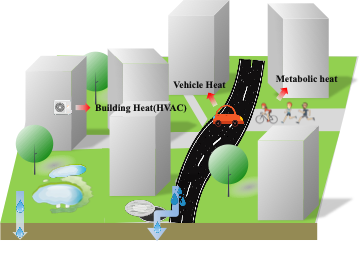
\includegraphics{Figures/城市模式/CoLM城市模式总体结构示意图.png}
\caption{CoLM城市模式总体结构示意图。}
\label{fig:CoLM城市模式总体结构示意图}
\end{figure}
}

建筑物底面考虑为正方形,边长为记为$L$。在已知$f_b$和$H/W$参数时,$L$可以计算为:
\begin{equation}
\frac{H}{L}=\frac{H}{W} \cdot \frac{1-\sqrt{f_{b}}}{\sqrt{f_{b}}}, \text { 即 } L=W \frac{\sqrt{f_{b}}}{1-\sqrt{f_{b}}}
\end{equation}
对于同一所在地城市覆盖,单栋建筑物几何参数一致,目前未考虑建筑物之间的几何差异,即以上参数代表为统计平均值。

在以下分模块公式推导中,下标约定如下:天空($s$),地面($g$,包括透水面$gper$和不透水面$gimp$),
墙面($w$,包括阳面墙$wsun$和阴面墙$wsha$),植被($v$)和屋顶$(r$)。$F$表示可视因子,例如$F_{gs}$表示从地面到天空的可视因子。
$S$表示阴影,$H/W$在推导过程中表示为$HW$,$H/L$表示为$HL$,总的直射入射和漫射入射太阳辐射能量通量采用单位能量1表示。

{
\begin{figure}[htbp]
\centering
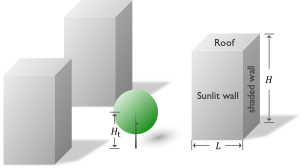
\includegraphics{Figures/城市模式/CoLM城市模式几何结构示意图.png}
\caption{CoLM城市模式几何结构示意图。}
\label{fig:CoLM城市模式几何结构示意图}
\end{figure}
}
\section{短波辐射传输}\label{短波辐射传输}
\subsection{无植被覆盖时短波辐射传输}\label{无植被覆盖时短波辐射传输}
太阳辐射直射照射时(太阳天顶角$\theta_s$),
建筑物群落在地面的阴影覆盖占比(被墙面遮挡的部分)计算为:
\begin{equation}\label{S_w}
S_{w}=1-\exp \left(-\frac{4}{\pi} \cdot \frac{f_{b}}{f_{g}} {HL} \cdot \tan \left(\theta_{s}\right)\right)
\end{equation}
阳面墙面积比例计算为:
\begin{equation}\label{f_wsun}
f_{wsun}=0.5 \cdot \frac{s_{w} f_{g}+f_{b}}{\frac{4}{\pi} f_{b} {HL} \tan \left(\theta_{s}\right)+f_{b}}
\end{equation}
阴面墙比例:
\begin{equation}\label{f_wsha}
f_{wsha}=1-f_{wsun}
\end{equation}
对于天空到墙面的可视因子$F_{sw}$,即天空漫射光源到达墙面的辐射部分,其计算类似与直射光在被墙面遮挡的面积比例:
\begin{equation}\label{f_Sw}
F_{S w}=1-\exp \left(-\frac{4}{\pi} \cdot \frac{f_{b}}{f_{g}} {HL} \cdot \tan \left(\theta_{s}^{*}\right)\right)
\end{equation}
其中$\theta_s^\ast$为漫射光情况下等效角度,可近似计算为:
\begin{equation}
\theta_{s}^{*}=\frac{53-10 \sqrt{\frac{f_{b}}{f_{g}} {HL}}}{180} \cdot \pi
\end{equation}
根据能量守恒,天空到达地面的可视因子$F_{sg}=1-F_{sw}$。
根据可视因子对称性,地面到达墙面和天空的可视因子$F_{gw}=F_{sw}$,$F_{gs}=F_{sg}$。
墙面到天空和地面的可视因子($F_{ws}$, $F_{wg}$)根据互易原理,满足如下关系:
\begin{equation}
F_{ws} \cdot 4 {HL} f_{b}=F_{s w} f_{g}
\end{equation}
\begin{equation}
F_{w g} \cdot 4 {HL} f_{b}=F_{s w} f_{g}
\end{equation}
由于太阳辐射在墙面垂直分布并不均匀,对上式进行简单调整,$F_{ws}$和$F_{wg}$计算为:
\begin{equation}
F_{ws}=0.75 F_{s w} \frac{f_{g}}{f_{b}} \frac{1}{2 {HL}}
\end{equation}
\begin{equation}
F_{w g}=0.25 F_{s w} \frac{f_{g}}{f_{b}} \frac{1}{2 {HL}}
\end{equation}
墙面到墙面的可视因子$F_{ww}=1-F_{ws}-F_{wg}$。

a. 直射入射太阳辐射

对于直射辐射太阳辐射,直射光到达阳面墙的辐射通量$E_{wsun}=S_w$,
到达阴面墙的辐射通量$E_{wsha}=0$,到达地面的辐射通量$E_g=1-E_{wsun}$,
其中$E_{gimp}=E_gf_{gimp}$,$E_{gper}=E_gf_{gper}$。
阳面墙、阴面墙、不透水面和透水面第一次散射辐射通量可分别计算为:
$E_{wsun}\alpha_w,E_{wsha}\alpha_w,E_{gimp}\alpha_{gimp},E_{gper}\alpha_{gper}$,
其中$\alpha$表示墙面、不透水面和透水面的反照率,不分区阳面和阴面,不区分漫射和直射照射,且反射后的辐射假设为漫射辐射。
设经过墙面地面之间多次散射,达到辐射平衡时的墙面和地面辐射出射通量为$M$,可建立如下辐射平衡方程:
\begin{landscape}
\begin{equation}
\begin{array}{l}
    M_{ {wsun }}=E_{wsun} \alpha_{w}+M_{wsun} F_{ww} f_{wsun} \alpha_{w}+M_{wsha} F_{ww} f_{wsun} \alpha_{w}+M_{gimp} F_{g w} f_{wsun} \alpha_{w}+M_{gper} F_{g w} f_{wsun} \alpha_{w} \\ 
    M_{wsha}=E_{wsha} \alpha_{w}+M_{wsha} F_{ww} f_{wsha} \alpha_{w}+M_{wsun} F_{ww} f_{wsha} \alpha_{w}+M_{gimp} F_{g w} f_{wsha} \alpha_{w}+M_{gper} F_{g w} f_{wsha} \alpha_{w} \\ 
    M_{gimp}=E_{gimp} \alpha_{gimp}+M_{wsun} F_{w g} f_{ gimp} \alpha_{gimp}+M_{wsha} F_{w g} f_{ gimp} \alpha_{gimp} \\ 
    M_{gper}=E_{gper} \alpha_{gper}+M_{wsun} F_{w g} f_{gper} \alpha_{gper}+M_{wsha} F_{w g} f_{gper} \alpha_{gper}
\end{array}
\end{equation}
通过整理得到:
\begin{equation}
\left(\begin{array}{cccc}1-F_{ww} f_{wsun} \alpha_{w} & -F_{ww} f_{wsun} \alpha_{w} & -F_{g w} f_{wsun} \alpha_{w} & -F_{g w} f_{wsun} \alpha_{w} \\
    -F_{ww} f_{wsha} \alpha_{w} & 1-F_{ww} f_{wsha} \alpha_{w} & -F_{g w} f_{wsha} \alpha_{w} & -F_{g w} f_{wsha} \alpha_{w} \\
    -F_{w g} f_{gimp} \alpha_{gimp} & -F_{w g} f_{gimp} \alpha_{gimp} & 1 & 0 \\ 
    -F_{w g} f_{gper} \alpha_{gper} & -F_{w g} f_{gper} \alpha_{gper} & 0 & 1\end{array}\right)
    \left(\begin{array}{l}M_{wsun} \\ M_{ {wsha }} \\ 
    M_{ gimp} \\ 
    M_{gper}\end{array}\right)=\left(\begin{array}{c}E_{wsun} \alpha_{w} \\
    E_{wsha} \alpha_{w} \\
    E_{gimp} \alpha_{ gimp} \\
    E_{gper} \alpha_{gper}\end{array}\right)
\end{equation}
\end{landscape}

简单表示为
\begin{equation}\label{mathbf_AX}
\mathbf{A X}=\mathbf{B}
\end{equation}
$\mathbf{A}$为辐射传输矩阵,$\mathbf{B}$为向量($E_{wsun}\alpha_w$,$E_{wsha}\alpha_w$,
$E_{gimp}\alpha_{gimp}$,$E_{gper}\alpha_{gper}$),
即墙面和地面第一次散射辐射通量。$\mathbf{X}$为求解变量组成的向量($M_{wsun}$,$M_{wsha}$,$M_{gimp}$,$M_{gper}$),
计算为:
\begin{equation}\label{mathbf_X}
\mathbf{X}=\mathbf{A}^{-1} \mathbf{B}
\end{equation}
矩阵$\mathbf{A}$是由已知变量组成的常数矩阵,可直接进行求逆计算,从而计算得到$\mathbf{X}$。墙面和地面的辐射吸收计算为:
\begin{equation}\label{s_wsun_wsha_gimp_gper_1}
\begin{array}{c}s_{wsun}=\frac{M_{wsun}}{\alpha_{w}}\left(1-\alpha_{w}\right) \\ 
    s_{wsha}=\frac{M_{wsha}}{\alpha_{w}}\left(1-\alpha_{w}\right) \\
    s_{gimp}=\frac{M_{gimp}}{\alpha_{gimp}}\left(1-\alpha_{gimp}\right) \\
    s_{gper}=\frac{M_{gper}}{\alpha_{gper}}\left(1-\alpha_{gper}\right)\end{array}
\end{equation}
注意,以上辐射吸收为总吸收量,其各自单面面积辐射吸收量修改为:
\begin{equation}\label{s_wsun_wsha_gimp_gper_2}
\begin{array}{c}s_{wsun}=\frac{f_{g}}{4 f_{wsun} \mathrm{HL} f_{b}} s_{wsun} \\ 
    s_{wsha}=\frac{f_{g}}{4 f_{wsha} \mathrm{HL} f_{b}} s_{wsha} \\ 
    s_{gimp}=\frac{1}{f_{gimp}} s_{gimp} \\ 
    s_{gper}=\frac{1}{f_{gper}} s_{gper}\end{array}
\end{equation}
不考虑屋顶时的城市反照率为:
\begin{equation}\label{alpha_u}
\alpha_{u}=M_{wsun} F_{ws}+M_{wsha} F_{ws}+M_{gimp} F_{gs}+M_{gper} F_{gs}
\end{equation}
屋顶的吸收计算为$s_{roof}=1-\alpha_{roof}$,考虑屋顶的城市反照率(\ref{alpha_u})修订为:
\begin{equation}\label{alpha_u2}
\alpha_{u}=\alpha_{{roof }} f_{b}+\alpha_{u} f_{g}
\end{equation}

b.漫射入射太阳辐射
对于漫射,计算过程与直射入射辐射过程基本类似,不同之处在于首次到达墙面和地面的辐射通量分别为:
$F_{sw}f_{wsun}$、$F_{sw}f_{wsha}$、$F_{sg}f_{gimp}$、$F_{sg}f_{gper}$,即公式(\ref{mathbf_AX})中的$\mathbf{B}$。
漫射入射辐射的传输矩阵同直射入射辐射情景,即A。其求逆后的结果可以直接用于漫射入射辐射,利用公式(\ref{mathbf_X})计算得到墙面和地面的辐射出射通量,
单位面积的辐射吸收和城市反照率同公式(\ref{alpha_u})和(\ref{alpha_u2}),在此不再列出。

\subsection{有植被覆盖时短波辐射传输}\label{有植被覆盖时短波辐射传输}
城市中考虑植被后的短波辐射传输过程是在无植被辐射传输的基础上,考虑植被在内的各组分之间的可视因子,
从而计算辐射平衡时的传输矩阵,采用类似的方法求解墙面、地面和植被的辐射吸收。
相比章节 \ref{无植被覆盖时短波辐射传输} 增加的部分为考虑植被在内的可视因子和阴影面积计算。

在植被树冠中心高度$h_v$处,墙面的阴影比例可根据公式(\ref{S_w})计算,利用$\frac{H-h_v}{H}$代替$HL$,记为$S_w^\prime$,即
\begin{equation}
S_{w}^{\prime}=1-\exp \left(-\frac{4}{\pi} \cdot \frac{f_{b}}{f_{g}} \frac{H-h_{v}}{H} \cdot \tan \left(\theta_{s}\right)\right)
\end{equation}
假设该阴影部分与植被覆盖$f_v$随机重叠,则植被被阴影遮挡的面积比例为$f_vS_w^\prime$,未覆盖的植被覆盖面积占比为$f_v^\prime=f_v-f_vS_w^\prime$。
该未被覆盖植被在整个城市覆盖区域的阴影覆盖$S_v$可根据公式(\ref{S_area})计算得到。将其覆盖比例转化为地面所占比例为:
\begin{equation}\label{S_v2}
S_{v}=S_{v} / f_{g}
\end{equation}

假设墙面在地面的阴影占比与植被的阴影随机重叠,则重叠部分占比$S_{vw}$计算为:
\begin{equation}
S_{v w}=S_{v}\left(S_{w}-S_{w}^{\prime}\right)
\end{equation}
该重叠部分假设全部为植被遮挡墙面部分。在地面覆盖区域,墙面的阴影占比修正为:
\begin{equation}\label{S_w2}
S_{w}=S_{w}-S_{v w}
\end{equation}
阴面墙和阳面墙的面积占比计算同公式(\ref{f_wsun})和(\ref{f_wsha})。

在不考虑植被存在时,可视因子$F_{sw}$, $F_{sg}$, $F_{gw}$, $F_{gs}$, $F_{ws}$, $F_{wg}$ 和 $F_{ww}$的
计算同章节 \ref{无植被覆盖时短波辐射传输},下面需要考虑植被的遮挡,对以上可视因子进行修改,并添加植被到各个面的可视因子。

同公式(\ref{S_v2})和(\ref{S_w2}),计算在漫射等效角度下的墙面和植被在地面的“阴影”占比(辐射遮挡) $S_w^\ast$和$S_v^\ast$,
利用公式(\ref{f_Sw})进行计算,则天空到达植被($F_{sv}$)、天空通过植被到墙面($F_{svw}$),以及天空通过植被到达地面的可视因子($F_{svg}$)分别计算为:
\begin{equation}\label{F_sv_svw_svg}
\begin{array}{c}F_{s v}=S_{v}^{*} \\ F_{s v w}=S_{v w}^{*} \\ F_{s v g}=F_{s v}-F_{s v w}\end{array}
\end{equation}
同理,地面到达植被($F_{gv}$)、地面通过植被到天空($F_{gvs}$),以及地面通过植被到达天空的可视因子($F_{gvs}$)可类似公式(\ref{F_sv_svw_svg})计算。

根据可视因子计算互易性原理,植被到天空、地面和墙面的可视因子计算为:
\begin{equation}
F_{vs}=F_{sv} \frac{f_g}{4 f_v}
\end{equation}
\begin{equation}
F_{vg}=F_{gv} \frac{f_g}{4 f_v}
\end{equation}
从而:
\begin{equation}
F_{v w}=1-F_{v s}-F_{v g}
\end{equation}
同理,根据互易性原理,$F_{wv}$计算为:
\begin{equation}
F_{w v}=F_{v w} \frac{f_{v}}{f_{b} \cdot {HL}}
\end{equation}
假设墙面通过植被到达墙面、天空和地面的可视因子与墙面到达相应各面的可视因子成正比,即:
\begin{equation}
F_{wvw}: F_{wvs}: F_{wvg}=F_{ww}: f_{1} F_{ws}: f_{2} F_{w g}
\end{equation}
其中$f_1=h_v/H$,$f_2=\left(H-h_v\right)/H$。根据能量守恒:
\begin{equation}
F_{wvw}+F_{wvs}+F_{wvg}=F_{w v}
\end{equation}
联合以上两式联立求解可得到:
\begin{equation}
F_{wvw}=\frac{F_{w v} F_{ww}}{F_{ww}+f_{1} F_{ws}+f_{2} F_{w g}}
\end{equation}
\begin{equation}
F_{wvs}=f_{1} \frac{F_{ws}}{F_{ww}} F_{wvw}
\end{equation}
\begin{equation}
F_{wvg}=f_{2} \frac{F_{w g}}{F_{ww}} F_{wvw}
\end{equation}
在此基础上,可以计算得到考虑植被影响的天空、墙面和地面之间的可视因子,
其中天空到墙面和地面的可视因子$F_{sw}^\prime$, $F_{sg}^\prime$计算为:
\begin{equation}
F_{s w}^{\prime}=F_{s w}-F_{s v w}+F_{s v w} T_{d}
\end{equation}
\begin{equation}
F_{s g}^{\prime}=F_{s g}-F_{s v g}+F_{s v g} T_{d}
\end{equation}
其中$T_d$为单棵球形树冠直射透射率,利用公式(\ref{T_ds_tau})计算。
地面到达墙面和天空的可视因子$F_{gw}^\prime$, $F_{gs}^\prime$计算为:
\begin{equation}
F_{g w}^{\prime}=F_{g w}-F_{g v w}+F_{g v w} T_{d}
\end{equation}
\begin{equation}
F_{gs}^{\prime}=F_{gs}-F_{g v s}+F_{g v s} T_{d}
\end{equation}
墙面到达地面、墙面和天空的可视因子$F_{wg}^\prime$, $F_{ww}^\prime$, $F_{ws}^\prime$计算为:
\begin{equation}
F_{w g}^{\prime}=F_{w g}-F_{wvg}+F_{wvg} T_{d}
\end{equation}
\begin{equation}
F_{ww}^{\prime}=F_{ww}-F_{wvw}+F_{wvw} T_{d}
\end{equation}
\begin{equation}
F_{ws}^{\prime}=F_{ww}-F_{wvs}+F_{wvs} T_{d}
\end{equation}

a. 直射入射太阳辐射

对于直射辐射太阳辐射,直射光到达阳面墙的辐射通量$E_{wsun}=S_w$,到达阴面墙的辐射通量$E_{wsha}=S_{vw}T_d$,
到达地面的辐射通量$E_g=1-S_w-S_v+\left(S_v-S_{vw}\right)T_d$,其中$E_{gimp}=E_gf_{gimp}$,$E_{gper}=E_gf_{gper}$,
$E_v=S_v$。阳面墙、阴面墙、不透水面、透水面和植被第一次散射辐射通量可分别计算为:$E_{wsun}\alpha_w$,$E_{wsha}\alpha_w$,
$E_{gimp}\alpha_{gimp}$,$E_{gper}\alpha_{gper}$,$E_v\alpha_v$,
其中$\alpha$表示反照率(对于植被表示所有向外散射辐射),不分区阳面和阴面,不区分漫射和直射照射,
且反射后的辐射假设为漫射辐射。假设经过墙面、地面和植被之间多次散射,达到辐射平衡时的墙面和地面辐射出射通量为$M$,
利用各组分之间的可视因子,可建立如下辐射平衡方程:
\begin{landscape}
\begin{equation}
\begin{array}{l}M_{wsun}=E_{wsun} \alpha_{w}+M_{wsun} F_{ww}^{\prime} f_{wsun} \alpha_{w}+M_{wsha} F_{ww}^{\prime} f_{wsun} \alpha_{w}+M_{gimp} F_{g w}^{\prime} f_{wsun} \alpha_{w}+M_{gper} F_{g w}^{\prime} f_{wsun} \alpha_{w}+M_{v} F_{v w} f_{wsun} \alpha_{w} \\ M_{wsha}=E_{wsha} \alpha_{w}+M_{wsha} F_{ww}^{\prime} f_{wsha} \alpha_{w}+M_{wsun} F_{ww}^{\prime} f_{wsha} \alpha_{w}+M_{gimp} F_{g w}^{\prime} f_{wsha} \alpha_{w}+M_{gper} F_{g w}^{\prime} f_{wsha} \alpha_{w}+M_{v} F_{v w} f_{wsha} \alpha_{w} \\ M_{gimp}=E_{gimp} \alpha_{gimp}+M_{wsun} F_{w g}^{\prime} f_{gimp} \alpha_{gimp}+M_{wsha} F_{w g}^{\prime} f_{gimp} \alpha_{gimp}+M_{v} F_{v g} f_{gimp} \alpha_{gimp} \\ M_{gper}=E_{gper} \alpha_{gper}+M_{wsun} F_{w g}^{\prime} f_{gper} \alpha_{gper}+M_{wsha} F_{w g}^{\prime} f_{gper} \alpha_{gper}+M_{v} F_{v g} f_{gper} \alpha_{gper} \\ M_{v}=E_{v} \alpha_{v}+M_{wsun} F_{w v} \alpha_{v}+M_{wsha} F_{w v} \alpha_{v}+M_{gimp} F_{g v} \alpha_{v}+M_{gper} F_{g v} \alpha_{v}\end{array}
\end{equation}
整理之后简化为:
\begin{equation}
\left(\begin{array}{ccccc}1-F_{ww}^{\prime} f_{wsun} \alpha_{w} & -F_{ww}^{\prime} f_{wsun} \alpha_{w} & -F_{g w}^{\prime} f_{wsun} \alpha_{w} & -F_{g w}^{\prime} f_{wsun} \alpha_{w} & -F_{v w} f_{wsun} \alpha_{w} \\ -F_{ww}^{\prime} f_{wsha} \alpha_{w} & 1-F_{ww}^{\prime} f_{wsha} \alpha_{w} & -F_{g w}^{\prime} f_{wsha} \alpha_{w} & -F_{g w}^{\prime} f_{wsha} \alpha_{w} & -F_{v w} f_{wsha} \alpha_{w} \\ -F_{w g}^{\prime} f_{gimp} \alpha_{gimp} & -F_{w g}^{\prime} f_{gimp} \alpha_{gimp} & 1 & 0 & -F_{v g} f_{gimp} \alpha_{gimp} \\ -F_{w g}^{\prime} f_{gper} \alpha_{gper} & -F_{w g}^{\prime} f_{gper} \alpha_{gper} & 0 & 1 & -F_{v g} f_{gper} \alpha_{gper} \\ -F_{w v} \alpha_{v} & -F_{w v} \alpha_{v} & -F_{g v} \alpha_{v} & -F_{g v} \alpha_{v} & 1\end{array}\right)\left(\begin{array}{c}M_{wsun} \\ M_{wsha} \\ M_{gimp} \\ M_{gper} \\ M_{v}\end{array}\right)=\left(\begin{array}{c}E_{wsun} \alpha_{w} \\ E_{wsha} \alpha_{w} \\ E_{gimp} \alpha_{gimp} \\ E_{gper} \alpha_{gper} \\ E_{v} \alpha_{v}\end{array}\right)
\end{equation}
\end{landscape}
方程求解同公式(\ref{mathbf_X}),阳面墙、阴面墙、不透水面和透水面的辐射总吸收及单位面积吸收同式(\ref{s_wsun_wsha_gimp_gper_1})和(\ref{s_wsun_wsha_gimp_gper_2})。植被的吸收计算类似,表达式为:
\begin{equation}
s_{v}=\frac{M_{v}}{a_{v}}\left(1-a_{v}-T_{d}\right)
\end{equation}
若考虑单位面积植被覆盖吸收辐射量,则$s_v$修订为:
\begin{equation}
s_{v}=\frac{f_{g}}{f_{v}} s_{v}
\end{equation}
不考虑屋顶时的城市反照率为:
\begin{equation}\label{alpha_u_a1}
\alpha_{u}=M_{wsun} F_{ws}^{\prime}+M_{wsha} F_{ws}^{\prime}+M_{gimp} F_{gs}^{\prime}+M_{gper} F_{gs}^{\prime}+M_{v} F_{v s}
\end{equation}
屋顶的吸收计算为$s_{roof}=1-\alpha_{roof}$,考虑屋顶的城市反照率(\ref{alpha_u_a1})修订为:
\begin{equation}
\alpha_{u}=\alpha_{roof} f_{b}+\alpha_{u} f_{g}
\end{equation}

b. 漫射入射太阳辐射

对于漫射,计算过程与直射入射辐射过程基本类似,不同之处在于首次到达墙面、地面和植被的辐射通量分别为:$F_{sw}^\prime f_{wsun}$、
$F_{sw}^\prime f_{wsha}$、$F_{sg}^\prime f_{gimp}$、$F_{sg}^\prime f_{gper}$和$F_{sv}$。
漫射入射辐射的传输矩阵同直射入射辐射情景。其求逆后的结果可以直接用于漫射入射辐射,各组分的辐射吸收和反照率计算过程在此不再赘述。 
\section{长波辐射传输}
\subsection{无植被覆盖时长波辐射传输}
无植被时的长波辐射传输类似与无植被时短波辐射传输时的漫射入射情景(长波辐射近似为漫射光源处理)。首次达到各组分表面的长波辐射通量为:
\begin{equation}
\begin{aligned} I_{wsun} &=L_{W} F_{s w} f_{wsun} \\ I_{wsha} &=L_{W} F_{s w} f_{wsha} \\ I_{gimp} &=L_{W} F_{s g} f_{gimp} \\ I_{gper} &=L_{W} F_{s g} f_{gper} \end{aligned}
\end{equation}
第一次反射的长波辐射通量依次分别为:
\begin{equation}
\begin{array}{c}I_{wsun}\left(1-\varepsilon_{w}\right) \\ I_{wsha}\left(1-\varepsilon_{w}\right) \\ I_{gimp}\left(1-\varepsilon_{gimp}\right) \\ I_{gper}\left(1-\varepsilon_{gper}\right)\end{array}
\end{equation}
上式中$\varepsilon$表示发射率,$\varepsilon_w$,$\varepsilon_{gimp}$,$\varepsilon_{gper}$为已知变量。各组分表面向外发射的长波辐射量为:
\begin{equation}
\begin{array}{c}4 f_{wsun} \mathrm{HL} \times \frac{f_{b}}{f_{g}} \times \sigma \varepsilon_{w} T_{wsun}^{4} \\
4 f_{wsha} \mathrm{HL} \times \frac{f_{b}}{f_{g}} \times \sigma \varepsilon_{w} T_{wsha}^{4} \\
\sigma \varepsilon_{gimp} T_{gimp}^{4} f_{gimp} \\
\sigma \varepsilon_{gper} T_{gper}^{4} f_{gper}\end{array}
\end{equation}
$T$表示温度,$\sigma$为斯蒂芬-玻尔兹曼常数。类似与短波辐射传输,可以构建辐射平衡方程:
\begin{landscape}
\begin{equation}
    \begin{aligned}
        L_{wsun}^{\uparrow}=I_{wsun}\left(1-\varepsilon_{w}\right)+L_{wsun}^{\uparrow} F_{ww} f_{wsun}\left(1-\varepsilon_{w}\right)+L_{wsha}^{\uparrow} F_{ww} f_{wsun}\left(1-\varepsilon_{w}\right)+L_{gimp}^{\uparrow} F_{g w} f_{wsun}\left(1-\varepsilon_{w}\right)\\+L_{gper}^{\uparrow} F_{g w} f_{wsun}\left(1-\varepsilon_{w}\right)+4 f_{wsun} H L * \frac{f_{b}}{f_{g}} * \sigma \varepsilon_{w} T_{wsun}^{4}\\
        L_{wsha}^{\uparrow}=I_{wsha}\left(1-\varepsilon_{w}\right)+L_{wsha}^{\uparrow} F_{ww} f_{wsha}\left(1-\varepsilon_{w}\right)+L_{wsun}^{\uparrow} F_{ww} f_{wsha}\left(1-\varepsilon_{w}\right)+L_{gimp}^{\uparrow} F_{g w} f_{wsha}\left(1-\varepsilon_{w}\right)\\+L_{gper}^{\uparrow} F_{g w} f_{wsha}\left(1-\varepsilon_{w}\right)+4 f_{wsha} H L * \frac{f_{b}}{f_{g}} * \sigma \varepsilon_{w} T_{wsha}^{4}\\
        L_{gimp}^{\uparrow}=I_{gimp}\left(1-\varepsilon_{gimp}\right)+L_{wsun}^{\uparrow} F_{w g} f_{gimp}\left(1-\varepsilon_{gimp}\right)+L_{wsha}^{\uparrow} F_{w g} f_{gimp}\left(1-\varepsilon_{gimp}\right)+\sigma \varepsilon_{gimp} T_{gimp}^{4} f_{gimp}\\
        L_{gper}^{\uparrow}=I_{gper}\left(1-\varepsilon_{gper}\right)+L_{wsun}^{\uparrow} F_{w g} f_{gper}\left(1-\varepsilon_{gper}\right)+L_{wsha}^{\uparrow} F_{w g} f_{gper}\left(1-\varepsilon_{gper}\right)+\sigma \varepsilon_{gper} T_{gper}^{4} f_{gper}
    \end{aligned}
\end{equation}
其中$L^\uparrow$表示各组分表面总的向外长波辐射量(反射部分+自身发射部分)。经过整理,可得:
\begin{equation}
\begin{aligned}
\left(\begin{matrix}1-F_{ww}f_{wsun}\left(1-\varepsilon_w\right)&-F_{ww}f_{wsun}\left(1-\varepsilon_w\right)&-F_{gw}f_{wsun}\left(1-\varepsilon_w\right)&-F_{gw}f_{wsun}\left(1-\varepsilon_w\right)\\-F_{ww}f_{wsha}\left(1-\varepsilon_w\right)&1-F_{ww}f_{wsha}\left(1-\varepsilon_w\right)&-F_{gw}f_{wsha}\left(1-\varepsilon_w\right)&-F_{gw}f_{wsha}\left(1-\varepsilon_w\right)\\-F_{wg}f_{gimp}\left(1-\varepsilon_{gimp}\right)&-F_{wg}f_{gimp}\left(1-\varepsilon_{gimp}\right)&1&0\\-F_{wg}f_{gper}\left(1-\varepsilon_{gper}\right)&-F_{wg}f_{gper}\left(1-\varepsilon_{gper}\right)&0&1\\\end{matrix}\right)
\left(\begin{matrix}L_{wsun}^\uparrow\\L_{wsha}^\uparrow\\L_{gimp}^\uparrow\\L_{gper}^\uparrow\\\end{matrix}\right)\\
=\left(\begin{matrix}I_{wsun}\left(1-\varepsilon_w\right)+2f_{wsun}\frac{\sigma\varepsilon_wT_{wsun}^4H}{W}\\I_{wsha}\left(1-\varepsilon_w\right)+2f_{wsha}\frac{\sigma\varepsilon_wT_{wsha}^4H}{W}\\I_{gimp}\left(1-\varepsilon_{gimp}\right)+\sigma\varepsilon_{gimp}T_{gimp}^4f_{gimp}\\I_{gper}\left(1-\varepsilon_{gper}\right)+\sigma\varepsilon_{gper}T_{gper}^4f_{gper}\\\end{matrix}\right)
\end{aligned}
\end{equation}
\end{landscape}

以上方程也可以记为矩阵形式:
\begin{equation}
\mathbf{A X}=\mathbf{B}
\end{equation}
求解以上方程得到$\mathbf{X}$,各组分表面长波净辐射量为:
\begin{equation}\label{L_wsun_wsha_gimp_pger_1}
\begin{array}{c}L_{wsun}=\frac{\varepsilon L_{wsun}^{\uparrow}-4 f_{wsun} \mathrm{HL} * \frac{f_{b}}{f_{g}} * \sigma \varepsilon_{w} T_{wsun}^{4}}{1-\varepsilon_{w}} \\ L_{wsha}=\frac{\varepsilon L_{wsha}^{\uparrow}-4 f_{wsha} \mathrm{HL} * \frac{f_{b}}{f_{g}} * \sigma \varepsilon_{w} T_{wsha}^{4}}{1-\varepsilon_{w}} \\ L_{gimp}=\frac{\varepsilon L_{w gimp}^{\uparrow}-\sigma \varepsilon_{gimp} T_{gimp}^{4} f_{gimp}}{1-\varepsilon_{gimp}} \\ L_{p g e r}=\frac{\varepsilon L_{w gper}^{\uparrow}-\sigma \varepsilon_{gper} T_{gper}^{4} f_{gper}}{1-\varepsilon_{gper}}\end{array}
\end{equation}
转化为单位面积净辐射时上式修改为:
\begin{equation}\label{L_wsun_wsha_gimp_pger_2}
\begin{array}{c}L_{wsun}=\frac{f_{g}}{4 f_{wsun} \mathrm{HL} f_{b}} L_{wsun} \\ L_{wsha}=\frac{f_{g}}{4 f_{wsha} \mathrm{HL} f_{b}} L_{wsha} \\ L_{gimp}=\frac{1}{f_{gimp}} L_{gimp} \\ L_{gper}=\frac{1}{f_{gper}} L_{gper}\end{array}
\end{equation}
在不考虑屋顶时的向外长波辐射通量计算为:
\begin{equation}
L^{\uparrow}=L_{wsun}^{\uparrow} F_{ws}+L_{wsha}^{\uparrow} F_{ws}+L_{gimp}^{\uparrow} F_{gs}+L_{gper}^{\uparrow} F_{gs}
\end{equation}


\subsection{有植被覆盖时长波辐射传输}\label{有植被覆盖时长波辐射传输}
考虑植被覆盖时的长波辐射计算类似于有植被覆盖时的短波辐射传输,根据之前介绍的无植被时长波辐射传输平衡方程,可以写出有植被覆盖时: 
\begin{landscape}
\begin{equation}
    \begin{aligned}
    L_{{wsun }}^{\uparrow}=I_{{wsun }}\left(1-\varepsilon_{w}\right)+L_{wsun}^{\uparrow} F_{ww}^{\prime} f_{wsun}\left(1-\varepsilon_{w}\right)+L_{wsha}^{\uparrow} F_{ww}^{\prime} f_{wsun}\left(1-\varepsilon_{w}\right)+L_{gimp}^{\uparrow} F_{g w}^{\prime} f_{wsun}\left(1-\varepsilon_{w}\right)+L_{gper}^{\uparrow} F_{g w}^{\prime} f_{wsun}\left(1-\varepsilon_{w}\right)\\+L_{v}^{\uparrow} F_{v w} f_{wsun}\left(1-\varepsilon_{w}\right)+4 f_{wsun} H L * \frac{f_{b}}{f_{g}} * \sigma \varepsilon_{w} T_{wsun}^{4} \\
    L_{wsha}^{\uparrow}=I_{wsha}\left(1-\varepsilon_{w}\right)+L_{wsha}^{\uparrow} F_{ww}^{\prime} f_{wsha}\left(1-\varepsilon_{w}\right)+L_{wsun}^{\uparrow} F_{ww}^{\prime} f_{wsha}\left(1-\varepsilon_{w}\right)+L_{gimp}^{\uparrow} F_{g w}^{\prime} f_{wsha}\left(1-\varepsilon_{w}\right)+L_{gper}^{\uparrow} F_{g w}^{\prime} f_{wsha}\left(1-\varepsilon_{w}\right)\\+L_{v}^{\uparrow} F_{v w} f_{wsha}\left(1-\varepsilon_{w}\right)+4 f_{wsha} H L * \frac{f_{b}}{f_{g}} * \sigma \varepsilon_{w} T_{wsha}^{4}\\
    L_{gimp}^{\uparrow}=I_{gimp}\left(1-\varepsilon_{gimp}\right)+L_{wsun}^{\uparrow} F_{w g}^{\prime} f_{gimp}\left(1-\varepsilon_{gimp}\right)+L_{wsha}^{\uparrow} F_{w g}^{\prime} f_{gimp}\left(1-\varepsilon_{gimp}\right)+L_{v}^{\uparrow} F_{v g} f_{gimp}\left(1-\varepsilon_{gimp}\right)+\sigma \varepsilon_{gimp} T_{gimp}^{4} f_{gimp} \\
    L_{gper}^{\uparrow}=I_{gper}\left(1-\varepsilon_{gper}\right)+L_{wsun}^{\uparrow} F_{w g}^{\prime} f_{gper}\left(1-\varepsilon_{gper}\right)+L_{wsha}^{\uparrow} F_{w g}^{\prime} f_{gper}\left(1-\varepsilon_{gper}\right)+L_{v}^{\uparrow} F_{v g} f_{gper}\left(1-\varepsilon_{gper}\right)+\sigma \varepsilon_{{gpre }} T_{{gpre }}^{4} f_{{gpre }} \\
    L_{v}^{\uparrow}=4 f_{v} / f_{g} \sigma \varepsilon_{v} T_{v}^{4}
    \end{aligned}
\end{equation}
\end{landscape}

\begin{landscape}
上式中的$F$, $F^\prime$表示可视因子,同章节 \ref{有植被覆盖时短波辐射传输}。经过整理,可以得到:
\begin{equation}
    \begin{split}
    \left(\begin{matrix}1-\ F_{ww}^\prime f_{wsun}\left(1-\varepsilon_w\right)&-\ F_{ww}^\prime f_{wsun}\left(1-\varepsilon_w\right)&-F_{gw}^\prime f_{wsun}\left(1-\varepsilon_w\right)&-F_{gw}^\prime f_{wsun}\left(1-\varepsilon_w\right)&-F_{vw}f_{wsun}\left(1-\varepsilon_w\right)\\
    -\ F_{ww}^\prime f_{wsha}\left(1-\varepsilon_w\right)&1-\ F_{ww}^\prime f_{wsha}\left(1-\varepsilon_w\right)&-F_{gw}^\prime f_{wsha}\left(1-\varepsilon_w\right)&-F_{gw}^\prime f_{wsha}\left(1-\varepsilon_w\right)&-F_{vw}f_{wsha}\left(1-\varepsilon_w\right)\\
    -F_{wg}^\prime f_{gimp}\left(1-\varepsilon_{gimp}\right)&-F_{wg}^\prime f_{gimp}\left(1-\varepsilon_{gimp}\right)&1&0&-F_{vg}f_{gimp}\left(1-\varepsilon_{gimp}\right)\\
    -F_{wg}^\prime f_{gper}\left(1-\varepsilon_{gper}\right)&-F_{wg}^\prime f_{gper}\left(1-\varepsilon_{gper}\right)&0&1&-F_{vg}f_{gper}\left(1-\varepsilon_{gper}\right)\\
    0&0&0&0&1\\\end{matrix}\right)\cdot \\
    \left(\begin{matrix}L_{wsun}^\uparrow\\L_{wsha}^\uparrow\\L_{gimp}^\uparrow\\L_{gper}^\uparrow\\L_v^\uparrow\\\end{matrix}\right)
    =\left(\begin{matrix}I_{wsun}\left(1-\varepsilon_w\right)+4f_{wsun}HL \times \frac{f_b}{f_g} \times \sigma\varepsilon_wT_{wsun}^4 \\
        I_{wsha}\left(1-\varepsilon_w\right)+4f_{wsha}HL \times \frac{f_b}{f_g} \times \sigma\varepsilon_wT_{wsha}^4  \\
        I_{gimp}\left(1-\varepsilon_{gimp}\right)+\sigma\varepsilon_{gimp}T_{gimp}^4f_{gimp} \\
        I_{gper}\left(1-\varepsilon_{gper}\right)+\sigma\varepsilon_{gper}T_{gper}^4f_{gper}\\
        4f_v/f_g\sigma\varepsilon_vT_v^4\\\end{matrix}\right)
    \end{split}
\end{equation}
\end{landscape}

求解以上方程,墙面和地面长波净辐射及单位面积净辐射计算公式同(\ref{L_wsun_wsha_gimp_pger_1})和(\ref{L_wsun_wsha_gimp_pger_2})。植被净辐射吸收为:
\begin{equation}
L_{v}=\left(L_{wsun}^{\uparrow} F_{w v}+L_{wsha}^{\uparrow} F_{w v}+L_{gimp}^{\uparrow} F_{g v}+L_{gper}^{\uparrow} F_{g v}+L_{W} F_{s v}\right) \varepsilon_{v}-4 f_{v} / f_{g} \sigma \varepsilon_{v} T_{v}^{4}
\end{equation}
植被单位面积覆盖长波净辐射修改为:
\begin{equation}
L_{v}=\frac{f_{g}}{f_{v}} L_{v}
\end{equation}
不考虑屋顶时城市总的向外长波辐射计算为:
\begin{equation}
L^{\uparrow}=L_{wsun}^{\uparrow} F_{ws}^{\prime}+L_{wsha}^{\uparrow} F_{ws}^{\prime}+L_{gimp}^{\uparrow} F_{gs}^{\prime}+L_{gper}^{\uparrow} F_{gs}^{\prime}+L_{v}^{\uparrow} F_{v s}
\end{equation}
\section{湍流交换过程}
城市湍流交换过程与三维植被湍流交换过程类似,计算屋顶、墙面(阴、阳面)、地面和植被的感热、潜热交换量,
同样是基于相似性理论,建立每层(等效高度)通量守恒方程,联立求解。不同之处在于其粗糙度、迎风面积指数、
零平面位移高度、风速/湍流交换系数衰减系数、建筑表面边界层阻抗计算与植被有所不同。
下面就无植被覆盖和有植被覆盖时对不同于自然植被湍流交换过程的部分进行简要说明。
\subsection{无植被覆盖时湍流交换过程}
建筑物的零平面位移高度采用~\citet{macdonald1998improved}方案:
\begin{equation}
\frac{d}{H}=1+A^{-f_{b}}\left(f_{b}-1\right)
\end{equation}
其中$A$取值为4.43。迎风面积指数可以计算为:
\begin{equation}
\lambda_{f}=\frac{2}{\pi} \cdot H L \cdot f_{b} \int_{0}^{\frac{\pi}{2}}(\cos \theta+\sin \theta) d \theta=\frac{4}{\pi} \cdot H L f_{b}
\end{equation}
粗糙度计算为:
\begin{equation}
\frac{z_{0}}{H}=\left(1-\frac{d}{H}\right) \exp \left[-\left(0.5 \frac{c_{D}}{\kappa^{2}}\left(1-\frac{d}{H}\right) \lambda_{f}\right)^{-0.5}\right]
\end{equation}
其中$C_D=1.2$,$\kappa=0.4$为 von K\'arman 常数。

城市冠层内的风速和湍流交换系数同样假设为指数衰减,但衰减系数与植被不同,
采用\citet{masson2000physically}方案,计算为0.5$HW$。建筑物(屋顶、墙面)边界层阻抗$r_b$计算为\citep{oleson2008urban}:
\begin{equation}
r_{b}=\frac{\rho_{a} c_{p}}{11.8+4.2 u_{e f f}}
\end{equation}
其中$u_{eff}$表示屋顶高度/墙面交换高度的等效风速值,$\rho_a$表示空气密度,$C_p$表示干空气定压比热容。

以上为主要区别于三维植被湍流交换过程计算的部分,整个正式湍流交换计算阻抗网络如图~\ref{fig:无植被覆盖时城市湍流交换阻抗示意图} 所示。
湍流交换计算过程与三维植被湍流交换方案类似,先通过相似性理论计算屋顶高度风速和湍流交换系数;
然后根据指数衰减假设,参考三维植被湍流交换方案~\citep{dai2019different},
根据公式(\ref{uz})和(\ref{Kz})计算风速和湍流交换系数在城市冠层内部剖面。屋顶的等效风速即为H高度时的风速,
墙面的等效风速为H到地面的平均风速,通过风速剖面积分计算得到。同理,屋顶与墙面等效交换高度之间的动力学交换阻抗,
以及墙面等效交换高度与地面之间的动力学阻抗$r_d$均是通过对交换系数剖面积分计算得到(公式(\ref{r_d1}))。
同多层植被湍流交换计算一样,对上图所示的屋顶和墙面等效交换高度建立感热和潜热通量守恒方程,
迭代求解其高度处的空气温度、湿度以及相似性理论交换长度(即空气不稳定程度)。
因为这部分过程与三维植被湍流交换过程完全一致,在此不再阐述。
{
\begin{figure}[htbp]
\centering
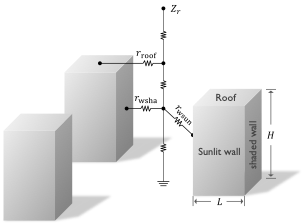
\includegraphics{Figures/城市模式/无植被覆盖时城市湍流交换阻抗示意图.png}
\caption{无植被覆盖时城市湍流交换阻抗示意图。}
\label{fig:无植被覆盖时城市湍流交换阻抗示意图}
\end{figure}
}


\subsection{有植被覆盖式湍流交换过程}
有植被覆盖时的湍流交换网络如图~\ref{fig:有植被覆盖时城市湍流交换阻抗示意图} 所示,
其计算过程与无植被覆盖时类似,不同之处在于新增植被组分。因此,在建立通量守恒方程式时,
需要考虑植被的感热、潜热交换,涉及到植被光合作用(蒸腾)和长波辐射吸收计算。
光合作用过程同自然植被光合作用过程,长波辐射吸收计算在章节 \ref{有植被覆盖时长波辐射传输} 已给出。
在实际计算过程中,可根据植被与建筑物高度差异,视情况分为两层或三层等效交换(三层时,即植被单独考虑为一层)。
整个过程也是迭代求解,但此时需要新增迭代求解变量叶片温度,其他过程同无植被覆盖时湍流交换过程。

{
\begin{figure}[htbp]
\centering
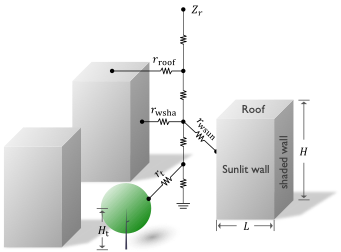
\includegraphics{Figures/城市模式/有植被覆盖时城市湍流交换阻抗示意图.png}
\caption{有植被覆盖时城市湍流交换阻抗示意图。}
\label{fig:有植被覆盖时城市湍流交换阻抗示意图}
\end{figure}
}


\section{城市温度传导计算}
城市内透水面、不透水面、墙面和屋顶的温度传导计算以自然界土壤温度传导计算为基础,基本过程一致,下面重点介绍城市的不同之处。

\subsection{透水面温度计算}
城市透水面即为土壤,与自然界土壤的热传递计算一致 (分层方案与土壤一致,
土壤热力参数也从全球数据中读取),只是上表面接收的短波、长波辐射及湍流交换通量(感热、潜热)由城市相应模块求解得到。

\subsection{不透水面温度计算}
不透水面的温度传导计算与透水面最大的不同之处在于需要将不透水面层的热力属性(导热率和热容)替换掉所在层的土壤热力属性。
另外在有雪、冰和水存在时,需要对第一层不透水面的热容进行订正。不透水面不考虑水分在内部的传递,相变过程只考虑第一层及以上积雪覆盖。

\subsection{墙面温度计算}
墙面(包括阴面墙、阳面墙)厚度从外部数据读取,同土壤一样,也分为10层,每层厚度一样,其热力参数从外部数据读取。
不同于透水面/不透水面,墙面不考虑积水、积雪覆盖,因此其热力属性完全由自身材料决定,同时也不考虑水传递、相变过程和潜热交换。

另一个不同之处在于最里(下)层的热量交换设置,对于土壤、不透水面,考虑最下一层无热量交换,但对于墙壁,
考虑室内墙壁表面温度与最里层墙壁的热量交换。除此之外,其他方面及其求解过程与土壤温度类似。


\subsection{屋顶温度计算}
屋顶的分层方案与墙壁一致。温度传递类似于墙面,但考虑屋顶积雪、积水覆盖时对屋顶第一层热力属性的影响,同不透水面。
同时最里层屋顶与室内屋顶表面温度考虑热量交换,相变过程只考虑第一层屋顶。


\section{城市水文过程}
对城市水文过程考虑主要分为三类:1) 透水面;2) 屋顶和不透水面;3) 城市水体。

对于透水面的处理同土壤水过程,计算产流和土壤水传输。对于城市水体,采用湖泊方案进行模拟。对于屋顶和不透水面,
考虑积雪和积水过程,类似与土壤积雪过程,但第一层为不透水面,液态水的最大承载量为不超过设定的值(max ponding),
超过的部分均当成地表产流处理。

由于目前城市水文过程比较简单,相应过程在土壤和湖泊模拟部分均有描述,在此不再赘述。


\section{城市人为热模拟}

\subsection{建筑能耗模型}
CoLM建筑物能耗模型如图~\ref{fig:建筑能耗模型示意图} 所示,同样是基于三维城市建筑群落结构假设,其过程类似于CLM5.0建筑能耗模型。
模型考虑墙体、屋顶的热传导过程,同时考虑室内空气与内墙壁、屋顶和室外的热量交换。根据室内设定的最高、
最低参考温度,来计算空调对应能耗,以感热的形式增加到湍流交换计算的源项中。
首先计算热交换通量并建立能量平衡方程,进而求解室内温度$T_{room}$,室内墙壁表面空气温度$T_{wsun,in}$,$T_{wsua,in}$和室内屋顶表面空气温度$T_{roof,in}$。
通量交换包括最里层墙壁/屋顶与屋内墙壁/屋顶表面空气热量交换,屋内墙壁/屋顶表面空气与室内空气热量交换以及室内空气与室外空气热量交换,通量平衡方程为: 

{
\begin{figure}[htbp]
\centering
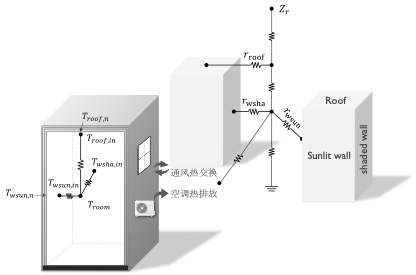
\includegraphics{Figures/城市模式/建筑能耗模型示意图.png}
\caption{建筑能耗模型示意图。}
\label{fig:建筑能耗模型示意图}
\end{figure}
}

\begin{landscape}
\begin{equation}
    \begin{array}{l}
        \begin{split}
        0.5 h_{{roof }, c v}\left(t_{{roof }, { in }}-t_{{room }}\right)+0.5 h_{{roof }, c v}\left(t_{{roof,in }}^{\prime}-t_{{room }}^{\prime}\right)=0.5 h_{{roof }, t k}\left(T_{{roof }, n}-T_{{roof }, { in }}\right)+0.5 h_{{roof }, t k}\left(T_{{roof }, n}-T_{{roof,in }}^{\prime}\right) \\
        0.5 h_{{wsun, }, v}\left(t_{{wsun,in }}-t_{{room }}\right)+0.5 h_{{wsun, cv }}\left(t_{wsun, i n}^{\prime}-t_{{room }}^{\prime}\right)=0.5 h_{{wsun,tk }}\left(T_{{wsun, } n}-T_{{wsun,in }}\right)+0.5 h_{{roof,tk }}\left(T_{{wsun, } n}-T_{{wsun,in }}^{\prime}\right)\\
        0.5 h_{wsha, c v}\left(t_{wsha, i n}-t_{{room }}\right)+0.5 h_{wsha, c v}\left(t_{wsha, i n}^{\prime}-t_{{room }}^{\prime}\right)=0.5 h_{wsha, t k}\left(T_{wsha, n}-T_{{roof }, i n}\right)+0.5 h_{wsha, t k}\left(T_{wsha, n}-T_{wsha, i n}^{\prime}\right)\\
        H \rho_{a} C_{p} \frac{T_{{room }}^{\prime}-T_{{room }}}{\Delta t}
        =\frac{ACH}{3600} H \rho_{a} C_{p}\left(T_{a f}-T_{{room }}^{\prime}\right)+0.5 h_{{roof }, c v}\left(t_{{roof }, { in }}-t_{{room }}\right)+0.5 h_{{roof }, c v}\left(t_{{roof }, { in }}^{\prime}-t_{{room }}^{\prime}\right)\\
        +0.5 h_{wsun, c v}\left(t_{wsun, i n}-t_{{room }}\right) f_{{wsun }}+0.5 h_{wsun, c v}\left(t_{wsun, i n}^{\prime}-t_{{room }}^{\prime}\right) f_{wsun} \\
        +0.5 h_{wsha, c v}\left(t_{wsha, i n}-t_{{room }}\right) f_{wsha}+0.5 h_{wsha, c v}\left(t_{wsha, i n}^{\prime}-t_{r o o m}^{\prime}\right) f_{wsha}
        \end{split}
    \end{array}
\end{equation}
以上方程组可写成矩阵形式:
\begin{equation}
    \begin{split}
\left(\begin{array}{cccc}0.5 h_{r o o f, c v}+0.5 h_{r o o f, t k} & 0 & 0 & -0.5 h_{r o o f, c v} \\ 0 & 0.5 h_{wsun, c v}+0.5 h_{wsun, t k} & 0 & -0.5 h_{wsun, c v} \\ 0 & 0 & 0.5 h_{wsha, c v}+0.5 h_{wsha, t k} & -0.5 h_{wsha, c v} \\ -0.5 h_{r o o f, c v} & -0.5 h_{wsun, c v} f_{wsun} & -0.5 h_{wsha, c v} f_{wsha} & \frac{H \rho_{a} C_{p}}{\Delta t}+\frac{{ ACH }}{3600} H \rho_{a} C_{p}\end{array}\right)
    \left(\begin{array}{c}T_{{roof,in }}^{\prime} \\ T_{wsun, i n}^{\prime} \\ T_{wsha, i n}^{\prime} \\ T_{{room }}^{\prime}\end{array}\right)=
    \\
    \left(\begin{array}{c}-0.5h_{roof,cv}\left(t_{roof,in}-t_{room}\right)+0.5h_{roof,tk}\left(T_{roof,n}-T_{roof,in}\right)+0.5h_{roof,tk}T_{roof,n}\\
        -0.5h_{wsun,cv}\left(t_{wsun,in}-t_{room}\right)+0.5h_{wsun,tk}\left(T_{wsun,n}-T_{wsun,in}\right)+0.5h_{wsun,tk}T_{wsun,n}\\
        -0.5h_{wsha,cv}\left(t_{wsha,in}-t_{room}\right)+0.5h_{wsun,tk}\left(T_{wsun,n}-T_{wsun,in}\right)+0.5h_{wsha,tk}T_{wsun,n}\\
        \frac{H \rho_{a} C_{p} T_{{room }}}{\Delta T}+\frac{ACH}{3600} H \rho_{a} C_{p} T_{a f}+0.5 h_{{roof,cv }}\left(t_{{roof,in }}-t_{{room }}\right)+0.5 h_{{wsun, cv }}\left(t_{{wsun,in }}-t_{{room }}\right) f_{{wsun }}+0.5 h_{{wsha,cv }}\left(t_{wsha, i n}-t_{{room }}\right) f_{{wsha }}  
    \end{array}\right)
    \end{split}
\end{equation}
\end{landscape}

上式中$T_{roof,in}^\prime$、$T_{wsun,in}^\prime$、$T_{wsha,in}^\prime$、$T_{room}^\prime$为需求解变量,其他变量均为已知量。
$T_{roof,in}$、$T_{wsun,in}$、$T_{wsha,in}$、$T_{room}$分别为上一时刻相应温度,
$T_{af}$为建筑室外空气温度。$h_{roof,cv}$、$h_{wsun,cv}$、$h_{wsha,cv}$
分别为室内屋顶表面空气、阳面、阴面墙表面空气与室内空气温度热交换系数,参考CLM5.0 \citep{oleson2020parameterization},$h_{roof,cv}=4.04$,
$h_{wsun,cv}=h_{wsha,cv}=3.076$。$ACH$为室内外空气热交换系数,设置为0.3。$T_{roof}$、$T_{wsun,n}$、$T_{wsha,n}$为最里层(用$n$表示)
屋顶、阴面墙、阳面墙的温度,为$h_{roof,tk}$、$h_{wsun,tk}$、$h_{wsha,tk}$为其与各自室内表面空气温度热交换系数,通过墙壁导热率和厚度计算得到。

以上方程组可通过矩阵求逆的方式进行求解,计算得到$T_{roof,in}^\prime$、$T_{wsun,in}^\prime$、
$T_{wsha,in}^\prime$、$T_{room}^\prime$。室内外热交换通量$F_{ach}$计算为:
\begin{equation}
F_{a c h}=\frac{ACH}{3600} H \rho_{a} C_{p}\left(T_{{room }}^{\prime}-T_{a f}\right)
\end{equation}
当$T_{room}^\prime>T_{room,max} $($T_{room,max}$为预设屋内最高温度,从外部数据读取)时,打开空调制冷,
使屋内温度维持在$T_{room,max}$,由此产生的空调热排放量$F_{hac}$为:
\begin{equation}
F_{{hac }}=H \rho_{a} C_{p} \frac{T_{{room }}^{\prime}-T_{{room,max }}}{\Delta t}
\end{equation}
当$T_{room}^\prime<T_{room,min}$ ($T_{room,min}$为预设屋内最高温度,从外部数据读取)时,
打开制暖设备,使屋内温度维持在$T_{room,min}$,由此产生的空调热排放量$F_{hac}$为:
\begin{equation}
F_{h a c}=H \rho_{a} C_{p} \frac{T_{{room }}^{\prime}-T_{{room,min }}}{\Delta t}
\end{equation}
在以上两种情况下,$T_{room}^\prime$更新为$T_{room,max}/T_{room,min}$。
由于制冷/制暖所浪费的热量排放分别计算为$0.6F_{hac}$和|$0.2F_{hac}$| (| |表示取绝对值)。
总的建筑热排放量为制冷/制暖热排放量加上其过程中浪费的热排放量。以上计算的热排放量均需乘以$f_b$来转化为单位城市面积通量,
并作为感热项 (源项) 加入到城市湍流交换平衡方程中,参考图~\ref{fig:建筑能耗模型示意图}。


\subsection{人体代谢热}
人体代谢热($Q_M$, \unit{W.m^{-2}})根据 \citet{allen2011} 的方法,按照能源清单法及 Top-Down 方法,利用人口密度数据,
将不同时刻的人体热排放映射到每个城市格点上,具体计算如下:
\begin{equation}
Q_{M}=P \cdot H_{M} \cdot 10^{-6}
\end{equation}
其中$P$为格点内人口密度(\unit{pop.km^{-2}}),目前使用的是 Gridded Population of the World (GPWv3) 数据,
分辨率为\ang{;2.5} (表~\ref{tab:人口密度数据}),$H_M$为不同时刻人体排放的热量。人体排放的热量遵循一个基本假设:
人在活动时每小时排放的热量为175 W (工作),非活动时排放量为75 W (休息),以及一个中间值125 W~\citep{sailor2004top};
除此之外,也没有考虑人口在不同格点间的移动。
% Please add the following required packages to your document preamble:
% \usepackage{booktabs}
\begin{table}[]
    \centering
    \caption{人口密度数据}
    \label{tab:人口密度数据}
    \begin{tabular}{@{}lll@{}}
    \toprule
    数据名称                            & 分辨率         & 来源                                                                                                     \\ \midrule
    Gridded Population of the World & \ang{;2.5}  & \begin{tabular}[c]{@{}l@{}}https://sedac.ciesin.columbia.edu/\\   data/collection/gpw-v3\end{tabular} \\ \bottomrule
    \end{tabular}
\end{table}


\subsection{交通热}
交通热排放($Q_v$, \unit{W.m^{-2}})同样根据~\citet{allen2011} 的方法利用能源清单法进行计算,
并采用Top-Down的方法,利用人口密度以及各个国家的汽车拥有量计算出格点内的汽车数量,
然后根据汽车行驶排放的热量以及交通流量的日分布计算出不同时刻的交通热排放。
其数据来源如表~\ref{tab:交通热数据及来源},具体计算方法如下:
\begin{equation}
Q_{v}=\frac{\left(V_{c} E_{c}+V_{M} E_{M}+V_{F R} E_{F R}\right) \cdot F \cdot 24 \cdot P \cdot D \cdot H_{t r a c}}{3.6 \cdot 10^{12}}
\end{equation}
% Please add the following required packages to your document preamble:
% \usepackage{booktabs}
\begin{table}[]
    \centering
\caption{交通热数据及来源}
\label{tab:交通热数据及来源}
    \begin{tabular}{@{}lll@{}}
    \toprule
    数据名称                       & 来源                          & Spatial/administrative unit   \\ \midrule
    Vehicles density and types & World mapper                & All countries and territories \\
    Daily vehicle pattern      & \citet{Hallenbeck1997} & All countries and territories \\
    Vehicle heat emissions     & \citet{smith2009estimating}       & All countries and territories \\ \bottomrule
    \end{tabular}
    \end{table}
其中$V_c$、$V_M$、$V_{FR}$分别为每千人拥有的汽车、摩托车、货车(巴士)的数量,该数据来自于World mapper
(\url{http://www.worldmapper.org/textindex/texttransport.htm});
$E_c$、$E_M$、$E_{FR}$则为三种机动车的排放系数,与机动车行驶速度有关,目前使用的 \citet{smith2009estimating} 的系数设置。
$F$为改变汽车数量的系数,相当于汽车总量的一部分在行驶,目前为固定系数(0.8);
$P$为格点内人口密度 (\unit{pop.km^{-2}});$D$为行驶的距离,同样与速度有关;$H_{trac}$为时间步长内交通流量分布。